% FIXED
\section{AAS from Accumulators}
\label{s:aas:construction}

This section presents our accumulator-based AAS construction.
We focus on bilinear accumulators here and discuss how our construction would benefit from RSA accumulators in \cref{s:aas:rsa}.
We give a more formal algorithmic description in \cref{s:aas:algorithms}.

As mentioned in \cref{s:intro:overview-techniques}, a bilinear accumulator over $n$ elements is already an AAS, albeit an inefficient one.
Specifically, proving (non)membership in a bilinear accumulator requires an $O(n)$ time polynomial division.
As a consequence, precomputing all $n$ membership proofs (naively) takes $O(n^2)$ time, which is prohibitive for most use cases.
Even worse, for non-membership, one must precompute proofs for all possible missing elements, of which there are exponentially many (in the security parameter $\lambda$).
Therefore, we need new techniques to achieve our desired polylogarithmic time complexity for computing both types of proofs in our AAS.

\parhead{A bilinear tree accumulator.}
Our first technique is to deploy the bilinear accumulator in a tree structure, as follows.
We start with the elements $e_i$ as leaves of a binary tree (see \cref{f:accumulated-tree}b).
Specifically, each leaf will store an accumulator over the singleton set $\{e_i\}$.
Every internal node in the tree will then store an accumulator over the union of the sets corresponding to its two children.
For example, the parent node of the two leaves corresponding to $\{e_i\}$ and $\{e_{i+1}\}$ stores the accumulator of the set $\{e_i,e_{i+1}\}$.
In this way, the root is the accumulator over the full set $S = \{e_1,\dots,e_n\}$ (see \cref{f:accumulated-tree}).
We stress that all these accumulators use the same public parameters.
The time to compute all the accumulators in the tree is $T(n) = 2T(n/2) + O(n\log{n}) = O(n\log^2{n})$ where $O(n\log{n})$ is the time to multiply the characteristic polynomials of two sets of size $n$ in the tree.
We call the resulting structure a \emph{bilinear tree} over set $S$.

\begin{figure}[t]
    \centering
    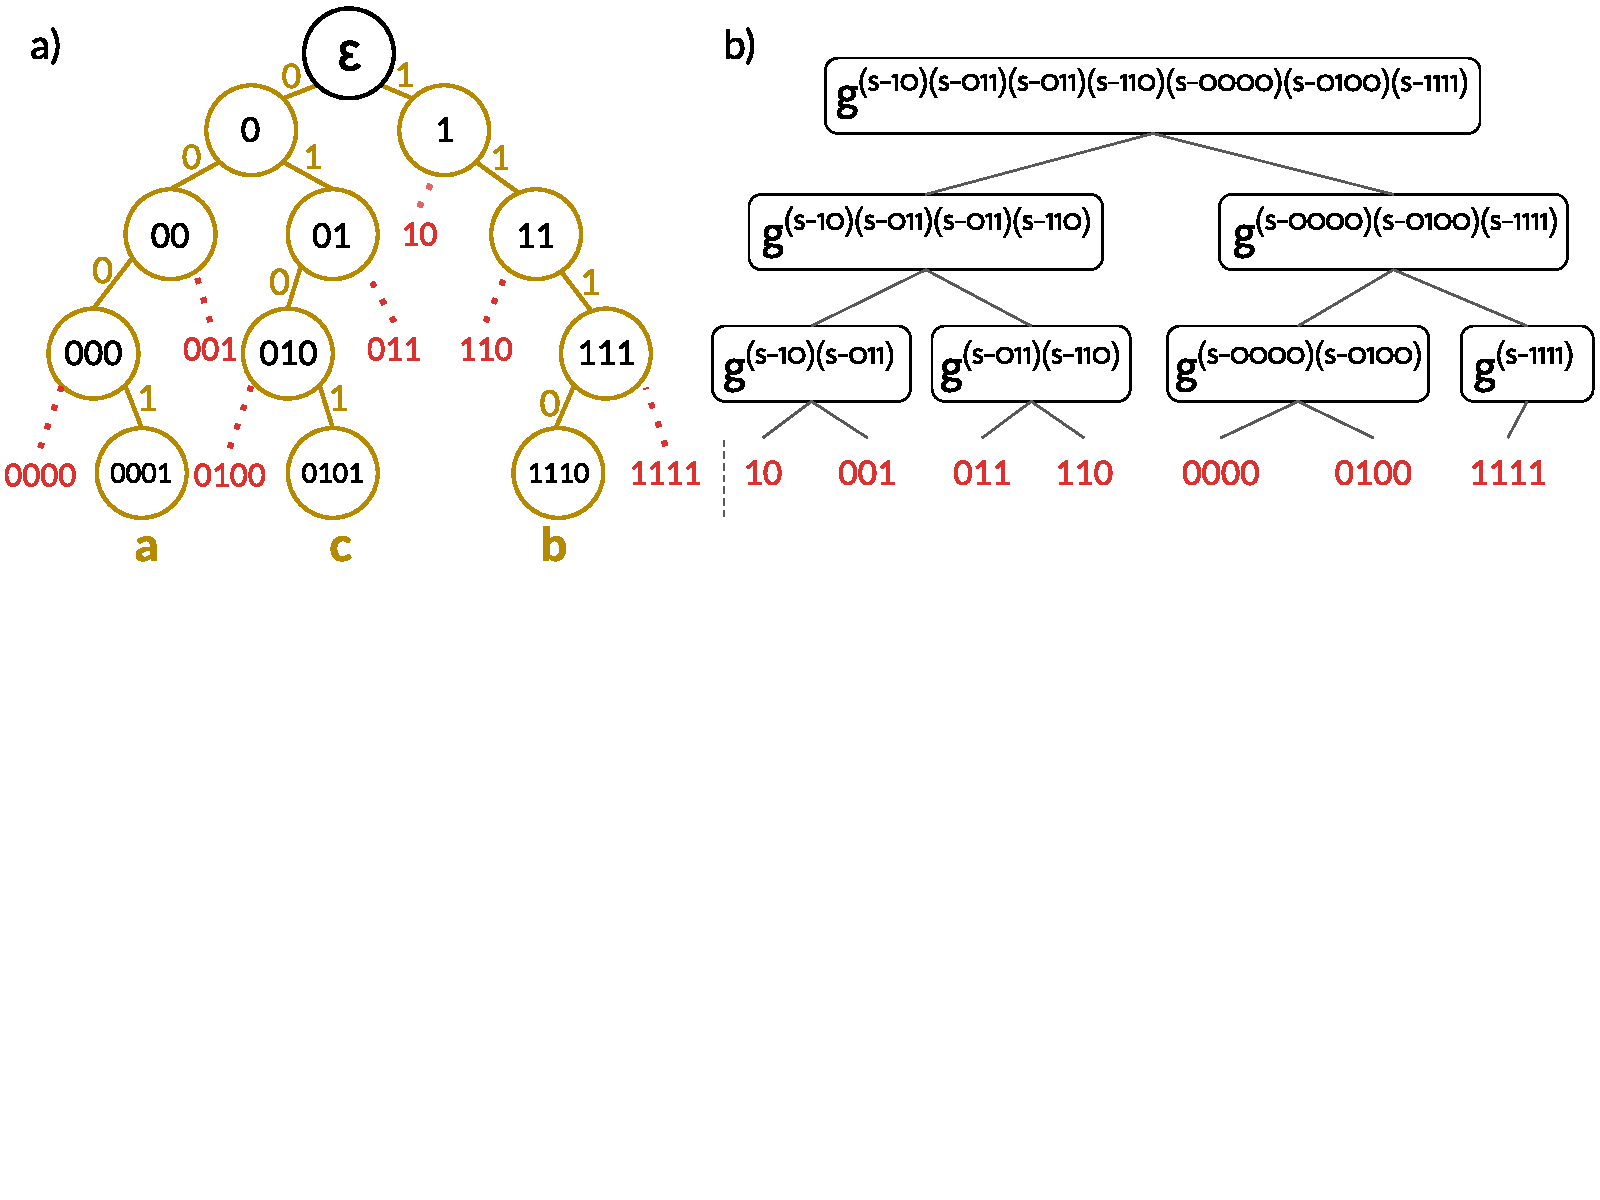
\includegraphics[width=1.00\columnwidth]{figures/AT.pdf}
    \vspace{-4.0cm}
    \caption{
        On the left side, we depict a trie over set $S = \{a,b,c\}$.
        Each element is mapped to a unique path of length $4$ in the trie.
        Nodes that are not in the trie but are at its \textit{frontier} are depicted in \myred{\textbf{red}}.
        On the right side, we depict a \textit{bilinear frontier tree} (BFT) corresponding to the set $S$.
        To prove that an element is not in $S$, we prove one of its prefixes is in the BFT.
        \label{f:accumulated-tree}}
    \vspace{-2.5em}
\end{figure}

\parhead{Membership proofs in bilinear trees.}
A membership proof for element $e_i$ will leverage the fact that sets along the path from $e_i$'s leaf to the root of the bilinear tree are subsets of each other.
The proof will consist of a sequence of \textit{subset proofs} that validate this (computed as explained in \cref{s:prelim:polycommit}).
Specifically, the proof contains the accumulators along the path from $e_i$'s leaf to the root, as well as the accumulators of all sibling nodes along this path (see \cref{f:accumulated-tree}b).
The client verifies all these subset proofs, starting from the singleton set $\{e_i\}$ in the leaf.
This convinces  him that $e_i$ is contained in the parent's accumulated set, which in turn is contained in its parent's accumulated set and so on, until the root.

Our bilinear tree approach gives us membership proofs of logarithmic size and thus logarithmic verification time.
Importantly, computing a bilinear tree in $O(n\log^2{n})$ time implicitly computes all membership proofs ``for free''!
In contrast, building a standard billinear accumulator over $S$ would yield constant-size proofs but in $O(n^2)$ time for all $n$ proofs.
Unfortunately, our bilinear tree structure does not (yet) support precomputing non-membership proofs.
We devise new techniques that address this next.

\parhead{Bilinear prefix trees to the rescue.}
To efficiently precompute non-membership proofs, we slightly modify our bilinear tree.
Instead of storing an element $e_i \in S$, the $i$th leaf will store the \emph{set of prefixes} of the binary representation of $e_i$.
We assume this representation is $2\lambda$ bits (or is made so using a CRHF) and can be mapped to an element in $\Fp$ (which is also of size $\approx 2\lambda$ bits) and thus can be accumulated.
For example, a leaf that previously stored element $e_1$ with binary representation $0001$, will now store the set $P(e_1) = \{\varepsilon,0,00,000,0001\}$ (i.e., all the prefixes of the binary representation of $e_1$, including the empty string $\varepsilon$).
In general, for each element $e_i$, $P(e_i)$ is the set of all $2\lambda+1$ prefixes of $e_i$.
Also, for any set $S = \{e_1,\dots,e_n\}$, we define its \emph{prefix set} as $P(S) = P(e_1) \cup \dots \cup P(e_n)$.
For example, let $S =\{a=0001,b=0101,c=1110\}$.
The root of $S$'s bilinear tree will contain an accumulator over $P(S) = P(a) \cup P(b) \cup P(c) = \{\varepsilon,0,1,00,01,11,000,010,111,0001,0101,1110\}$.

We refer to such a bilinear tree as a \emph{bilinear prefix tree (BPT)} over $S$.
The time to build a BPT for $S$ is $O(\lambda n\log^2{n})$ since there are $O(\lambda n)$ prefixes across all leaves.
Note that membership proofs in a BPT are the same as in bilinear trees, with a minor change.
The internal nodes of the tree still store accumulators over the union of their children.
However, the children now have common prefixes, which will only appear once in the parent.
For example, two children sets have the empty string $\varepsilon$ while their parent set only has $\varepsilon$ once (because of the union).
As a result, it is no longer the case that multiplying the characteristic polynomials of the children gives us the parent's polynomial.
Therefore, we can no longer rely on the siblings as subset proofs: we have to explicitly compute subset proofs for each child w.r.t. its parent.
We stress that this does not affect the asymptotic time complexity of computing the BPT.
As before, the client starts the proof verification from the leaf, which now stores a prefix set $P(e_i)$ rather than a singleton set $\{e_i\}$.

\begin{figure}[t]
    \centering
    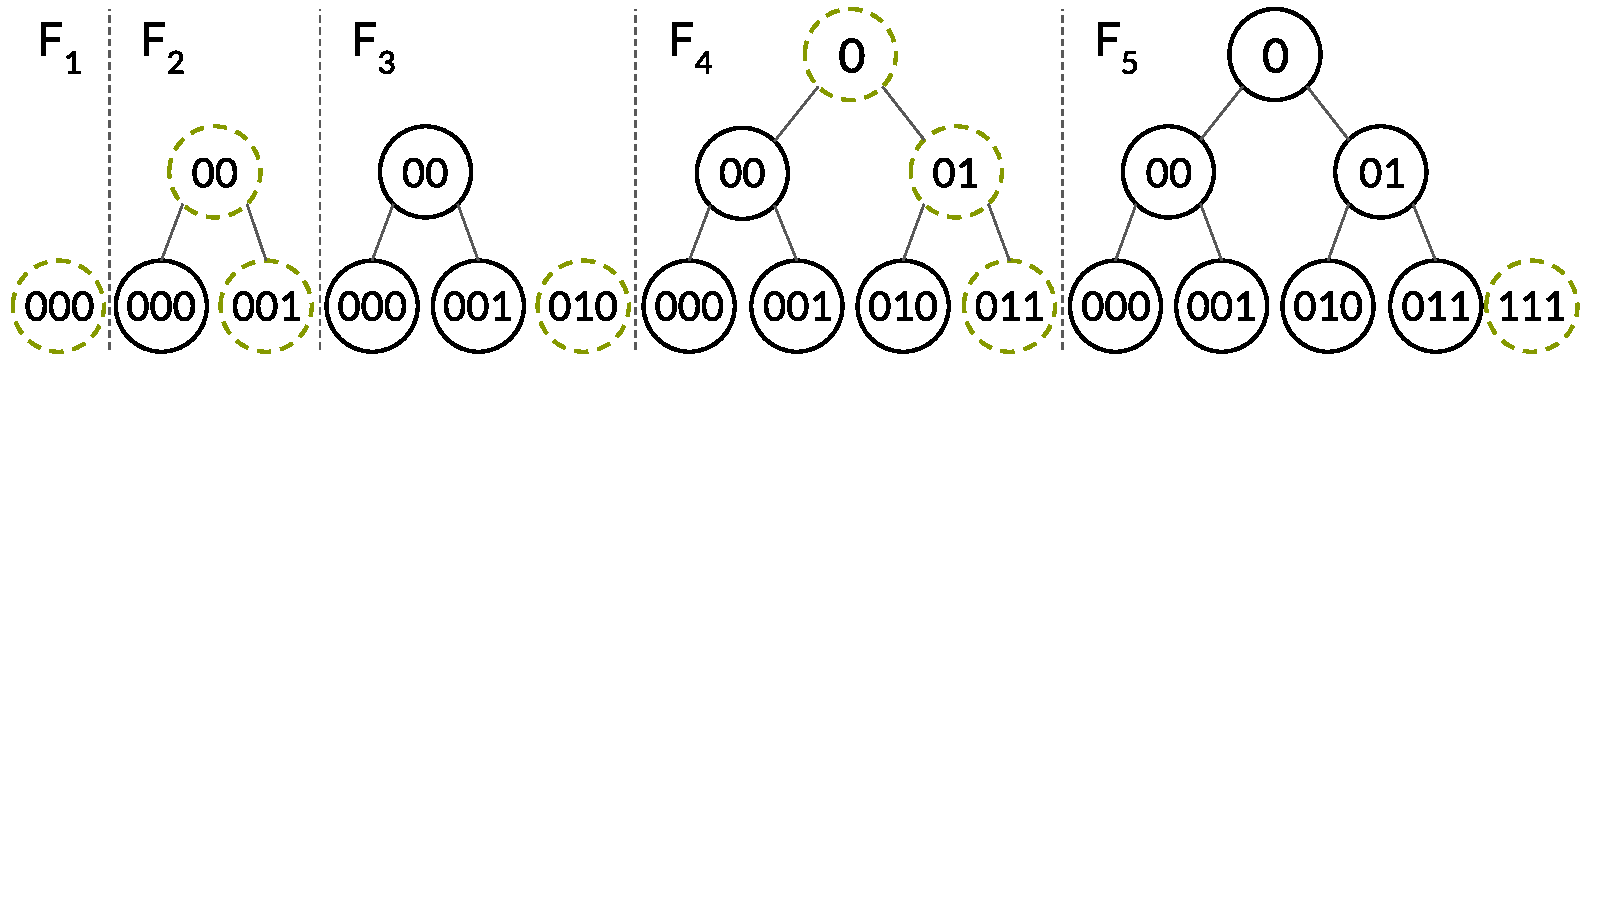
\includegraphics[width=1\columnwidth]{figures/forest.pdf}
    \vspace{-3.4cm}
    \caption{
        A forest starting empty and going through a sequence of five appends.
        A forest only has trees of exact size $2^j$ for distinct $j$'s.
        A forest of $n$ leaves has \textit{at most} $\log{n}$ trees. 
    }
    \label{f:forest}
    \vspace{-1.55em}
\end{figure}

\parhead{Efficient non-membership proofs.}
But how does a BPT help with precomputing non-membership proofs for any element $e'\notin S$?
First, note that, because of our use of prefixes, to prove $e'\notin S$ it suffices to show that \textit{any one prefix $\rho$ of $e'$ is not contained in $P(S)$}.
Second, note that there might exist other elements $e''$ who share $\rho$ as a prefix.
As a result, the non-membership proof for $e'$ could be ``reused'' as a non-membership proof for $e''$.
This is best illustrated in \cref{f:accumulated-tree}a using our previous example where $S =\{a,b,c\}$.
Consider elements $d= \underline{011}1$ and $f = \underline{011}0$ that are not in $S$.
To prove non-membership for either element, it suffices to prove the same statement: $\underline{011}\notin P(S)$.
Thus, if we can identify all such \textit{shared prefixes}, we can use them to prove the non-membership of (exponentially) many elements.
(This technique is also used in Micali et al.'s zero-knowledge sets~\cite{zks}.)

To do this, we insert all elements from $S$ in a trie as depicted in \cref{f:accumulated-tree}a.
Next, we keep track of the prefixes at the ``frontier'' of the trie depicted in red in \cref{f:accumulated-tree}a.
We immediately notice that to prove non-membership of any element, it suffices to prove non-membership of one of these \textit{frontier prefixes}!
In other words, elements that are not in $S$ will have one of these as a prefix.
Thus, we formally define the \textit{frontier} of $S$ as:
\begin{align*}
    F(S) &= \{\rho \in \{0,1\}^{\le 2\lambda}: {\rho\not \in P(S)} \wedge {\parent(\rho) \in P(S)}\}\text{,}
\end{align*}
where $\parent(\rho)$ is $\rho$ without its last bit (e.g., $\parent(011) = 01$).
Note that the size of $F(S)$ is $O(\lambda n)$, proportionate to $P(S)$.

Most importantly, from the way $P(S)$ and $F(S)$ are defined, for any element $e'$ it holds that $e'\not\in S$ if, and only if, some prefix of $e'$ is in $F(S)$. 
Therefore, proving non-membership of $e'$ boils down to proving two statements: (i) some prefix of $e'$ belongs to $F(S)$, and (ii) $P(S) \cap F(S) = \varnothing$.
We stress that the latter is necessary as a malicious server may try to craft $F(S)$ in a false way (e.g., by adding some prefixes both in $P(S)$ and in $F(S)$).
To prove (i), we build a bilinear tree over $F(S)$ which gives us precomputed membership proofs for all $\rho \in F(S)$.
We refer to this tree as the \emph{bilinear frontier tree (BFT)} for set $S$ and to the proofs as \textit{frontier proofs}.
To prove (ii), we compute a \emph{disjointness proof} between sets $P(S)$ and $F(S)$, as described in \cref{s:prelim:polycommit} (i.e., between the root accumulators of the BFT and the BPT of $S$).
The time to build a BFT for $S$ is $O(\lambda n\log^2{n})$ since $F(S)$ has $O(\lambda n)$ elements.
The disjointness proof can be computed in $O(\lambda n\log^2{n})$ time. 

\parhead{Static AAS construction.}
Combining all the above techniques, we obtain a \textit{static} AAS that does not support updates efficiently (nor append-only proofs).
This construction consists of: (a) a BPT for $S$, (b) a BFT for $S$, and (c) a proof of disjointness between $P(S)$ and $F(S)$ (i.e., between the root BPT and BFT accumulators).
The height of the BPT is $O(\log n)$ and the height of the BFT is $O(\log{(\lambda n)})$ so the size and verification time of a (non)membership proof is $O(\log{n})$.
The digest is just the root accumulator of the BPT. 

\begin{figure}[t]
    \centering
    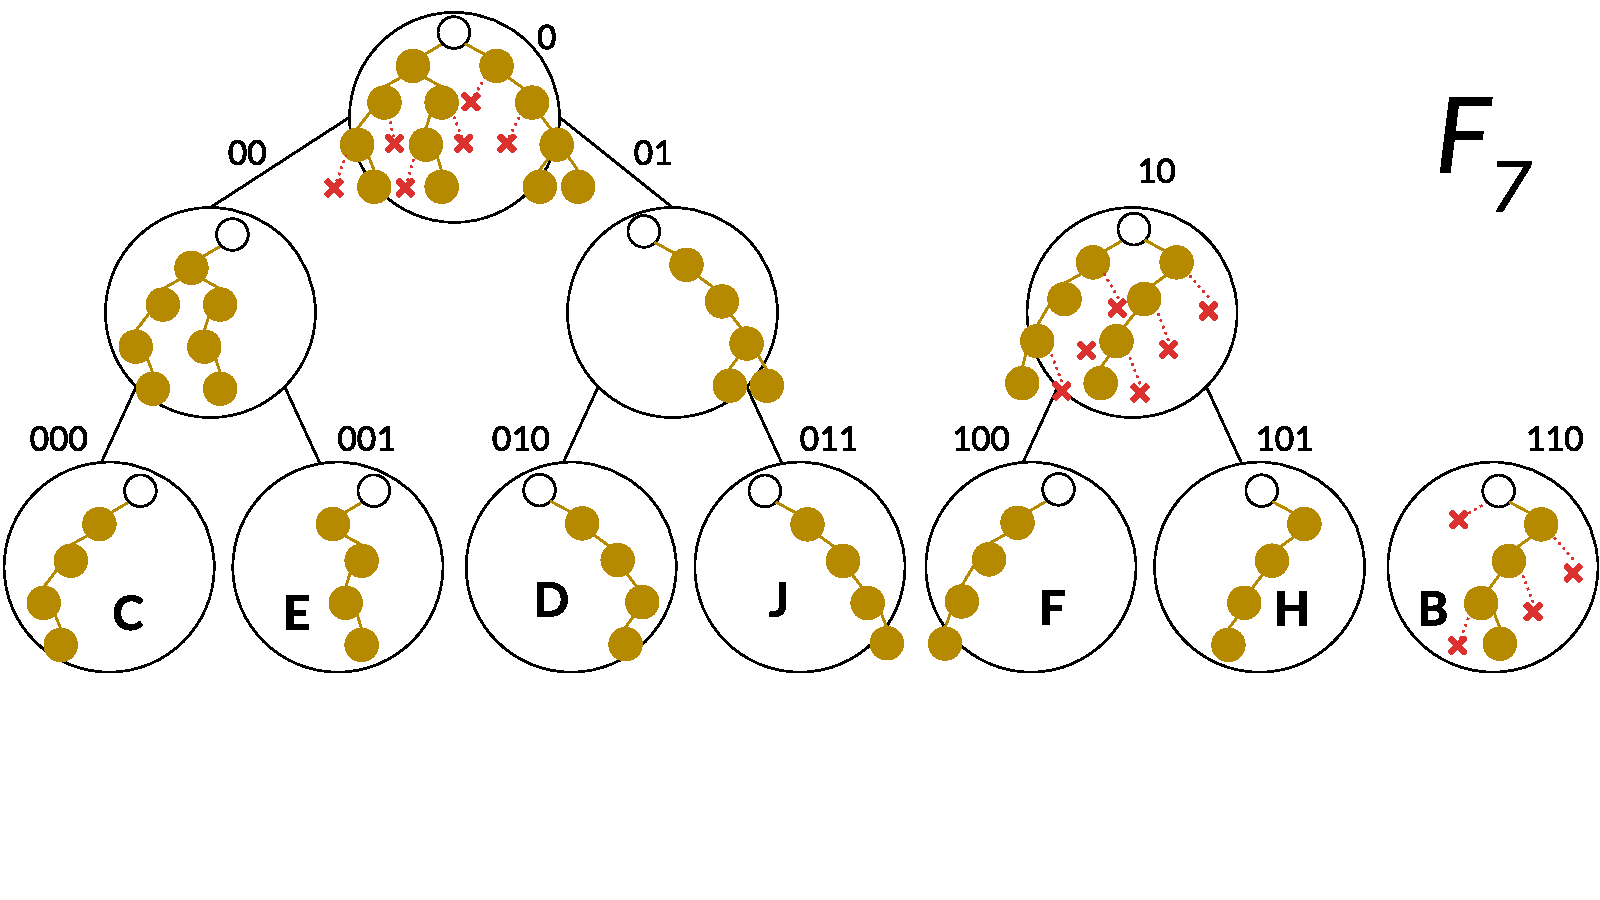
\includegraphics[width=1.00\columnwidth]{figures/accaad.pdf}
    \vspace{-1.7cm}
    \caption{
        A dynamic AAS with $\lambda=2$ for set $\{B,C,D,E,F,H,J\}$.
        Our AAS is a forest of BPTs with corresponding BFTs.
        Each node stores a BPT accumulator (and subset proof), depicted as a trie, in \myyellow{yellow}.
        Root nodes store a BFT, depicted as the missing \myred{red} nodes.
    }
    \vspace{-1.9em}
    \label{f:accaas}
\end{figure}

\parhead{Handling appends efficiently.}
So far, we only discussed the case of a static set $S$.
However, our AAS should support appending new elements to $S$. 
The main challenge here is \emph{efficiency} since updating the BPT and BFT as well as the disjointness proof after each update is very expensive (at least linear).
To address this we use a classic ``amortization'' trick from Overmars~\cite{overmars} also used in~\cite{distributed-acc}. 

Specifically, our AAS will consist not of one BPT for the entire set $S$, but will be partitioned into a \textit{forest} of BPTs and their corresponding BFTs.
Initially, we start with no elements in the AAS.
When the first element $e_1$ is appended, we build its \textit{tree-pair}: a BPT over the set $\{e_1\}$, its BFT and a disjointness proof.
When the second element $e_2$ is appended, we ``merge'': we build a size-2 tree-pair over $\{e_1, e_2\}$.
The rule is we always merge equal-sized tree-pairs.
When $e_3$ is appended, we cannot merge it because there's no other tree-pair of size 1.
Instead, we create a tree-pair over $\{e_3\}$.
In general, after $2^\ell - 1$ appends, we end up with $\ell$ separate tree-pairs corresponding to sets of elements $S_1,\dots,S_\ell$.
The final set is $S=\bigcup_{j=1}^{\ell} S_j$ where $|S_j| = 2^j$.
The evolution of such a forest is depicted in \cref{f:forest} and the final data structure can be seen in \cref{f:accaas}.

Let us analyze the time to merge two size-$n$ tree-pairs for $S_1$ and $S_2$ into a size-$2n$ tree-pair for $S=S_1 \cup S_2$.
To compute $S$'s BPT, we need to (i) compute its root accumulator, (ii) set its children to the ``old'' root accumulators of $S_1$ and $S_2$ and (iii) compute subset proofs $S_1 \subset S$ and $S_2\subset S$.
Since $|S_1|=|S_2|=n$, operations (i), (ii) and (iii) take $O(\lambda n \log^2{n})$ time.
Finally, we can compute $S$'s BFT from scratch in $O(\lambda n\log^2 n)$ time.

To analyze the append time, consider the time $T(n)$ to create an AAS over a set $S$ with $n = 2^\ell$ elements (without loss of generality).
Then, $T(n)$ is just the time to create a tree-pair over $S$ and can be broken into (i) the time to create a tree-pair over the children of $S$ of size $n/2$ (i.e., $2T(n/2)$) (ii) the time to merge these two children BPTs (including computing subset proofs) and (iii) the time to compute the BFT of $S$.
More formally, $T(n) = 2T(n/2) + O(\lambda n\log^2{n})$ which simplifies to $T(n) = O(\lambda n\log^3{n})$ time for $n$ appends.
Thus, the \textit{amortized} time for one append is $O(\lambda \log^3 {n})$ and can be de-amortized into \textit{worst-case} time using generic techniques~\cite{overmars,overmars-van-leeuwen}.

The downside of our amortized approach is that proving non-membership becomes slightly more expensive than in the static AAS data structure from above.
Specifically, now the server needs to prove non-membership in each tree-pair separately, requiring an $O(\log{n})$ frontier proof in each of the $O(\log{n})$ BFTs.
This increases the non-membership proof size to $O(\log^2 n)$.
On a good note, membership proofs remain unaffected: the server just sends a path to a leaf in \textit{one} of the BPTs where the element is found.
Finally, the AAS digest is set to the root accumulators of all BPTs and has size $O(\log{n})$.
We analyze the complexity of our AAS in \cref{s:aas:asymptotics}.

\parhead{Efficient append-only proofs.}
Our append-only proofs are similar to the ones in history trees~\cite{ht}.
% Recall that when we merge the BPTs for $S_1, S_2$ and build a new BPT, (i) we compute its new root as the accumulator of $P(S_1) \cup P(S_2)$, (ii) we set the two old roots as the new root's children and (iii) we compute subset proofs between the old roots and the new root.
% Thus, the old roots become children nodes in the new BPT.
% In fact, because every append to the AAS triggers a sequence of merges, we can generalize the above statement: after a sequence of appends, \textit{some} of the old roots in the old AAS will become descendants of a new root in the new AAS.
% The remaining old roots, if any, will remain as (new) roots in the new forest (e.g., root 0 from $F_4$ to $F_5$ in \cref{f:forest}).
% Our append-only proof leverages the above invariant.
An append-only proof must relate the root BPT accumulator(s) in the old AAS to the root BPT accumulator(s) in the new AAS.
We'll refer to these as ``old roots'' and ``new roots'' respectively.
Specifically, it must show that every old root either (i) became a new root or (ii) has a path to a new root with valid subset proofs at every level.
Such a path is verified by checking the subset proofs between every child and its parent, exactly as in a membership proof.
At the same time, note that there might be new roots that are neither old roots nor have paths to old roots (e.g., root 111 in $F_5$ from \cref{f:forest}).
The proof simply ignores such roots since they securely add new elements to the set.
To summarize, the append-only proof guarantees that each old root (1) has a valid subset path to a new root or (2) became a new root.

\parhead{Ensuring fork-consistency.}
For gossip protocols to work~\cite{ct-gossip,DahlbergPullsVestin2018}, our AAS must be fork-consistent.
Interestingly, append-only proofs do not imply fork-consistency.
For example, consider a server who computes an AAS for set $\{e_1\}$ and another one for the set $\{e_2\}$. 
The server gives the first set's digest to user $A$ and the second digest to user $B$.
Afterwards, he appends $e_2$ to the first set and $e_1$ to the second one, which ``joins'' the two sets into a common set $\{e_1,e_2\}$.
The append-only property was not violated (as the two users can deduce independently) but fork-consistency has been: the two users had diverging views that were subsequently merged.

To avoid this, we will ``Merkle-ize'' each BPT using a CRHF $\Hb$ in the standard manner (i.e., a node hashes its accumulator and its two children's hashes).
Our AAS digest is now set to the Merkle roots of all BPTs, which implicitly commit to all root accumulators in the BPTs.
As a result, after merging BPTs for elements $e_1$ and $e_2$, the Merkle root of the merged BPT will differ based on how appends were ordered: $(e_1,e_2)$, or $(e_2,e_1)$.
Thus, violating fork-consistency becomes as hard as finding a collision in $\Hb$ (see \cref{s:aas:proofs:fork-consistency}).
